The TRITIUM SiPMs are arranged in $4\times 4$ arrays. The electronics chosen to acquire and analyze the output signals of the SiPM arrays is PETsys \cite{PETSYS}, displayed in Figure \ref{fig:PETSYS}, which is a commercial system designed to work with SiPM arrays from Hamamatsu. PETsys provides time and energy digitalization, including QDCs\footnote{charge-to-digital converter} and TDCs\footnote{time-to-digital converter}. PETsys is a complete acquisition system capable of working with up to 1024 SiPM. This system consists of a basic board to which 16 different SiPM matrices can be connected with up to 64 SiPM per matrix. This number of channels is needed in the TRITIUM project because, as shown in section \ref{sec:TritiumMonitor}, the TRITIUM monitor consists of a large number of SiPM matrices with 16 channels per matrix.

\begin{figure}[h]
\centering
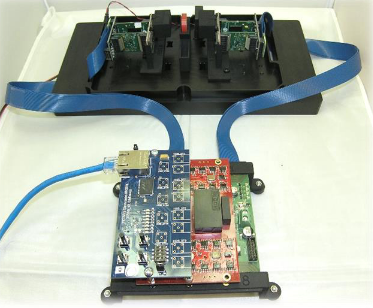
\includegraphics[scale=0.8]{3DesignPrinciples/32Tritium_detector/PETSYS_System.png}
\caption{Different parts of PETsys system\label{fig:PETSYS}~\cite{PETSYS}.}
\end{figure}
Although the capacity provided by PETsys should be enough for the requirements of the TRITIUM project, TRITIUM is a modular detector the sensitivity and background rejection capabilities of which could be improved by adding more modules with their corresponding photosensors. Therefore, the electronics should be scalable. This requeriment is fulfilled by PETsys since it has an additional module, called Clock and Trigger, to which up to $16$ different PETsys basic boards can be connected, which gives to PETsys a capacity of reading up to 256 SiPM matrices (16384 SiPMs). 

The PETsys software is based on C++ and Python scripts that drive the main tasks required, such as time coincidence options between SiPM (or even SiPM matrices) or energy discrimination. This software is open source, giving the possibility to modify the current scripts or to develop others with additional functions. PETsys has a time resolution better than $30~\pico\second$ which is one of the best time resolutions of commercial systems available and its price is around $10$\euro$/$ channel, which is cheaper than similar electronic systems. The PETsys system has the ability to monitor the temperature of the SiPM matrices and ASICS. In PETsys, the stabilization method of the SiPM gain reported in section \ref{sec:CharacterizationSiPM} can be implemented.

Some characterization measurements were carried out using the PETsys system to verify that the system works properly but the SiPM characterization was carried out at the level of a single channel (individual SiPM). The reason is that the output information of PETsys is already integrated and digitized, so it does not allow the SiPM to be calibrated. Therefore, to characterize a SiPM, a different electronic system was used to read up to eight different SiPMs. This system consists of a PCB that provides the SiPM bias voltage and reads the SiPM output signal. 

\begin{figure}
\centering
    \begin{subfigure}[b]{0.5\textwidth}
    \centering
    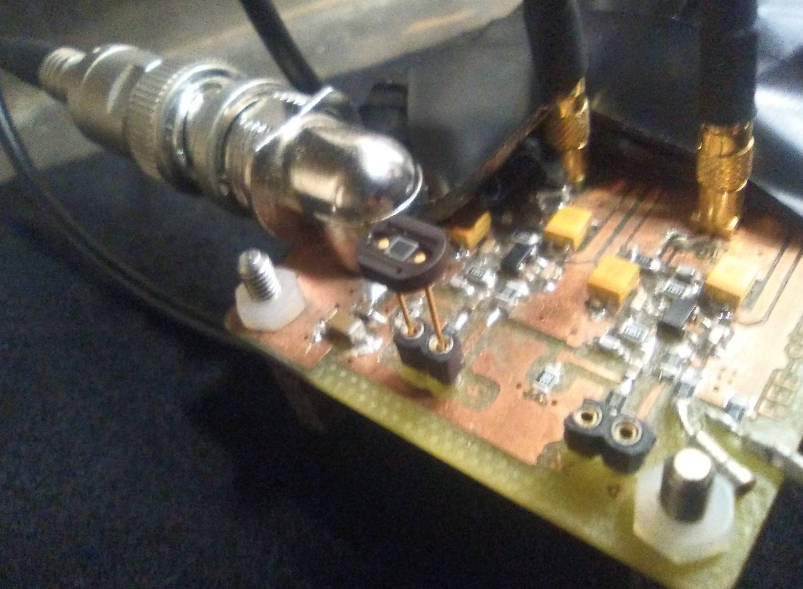
\includegraphics[width=\textwidth]{3DesignPrinciples/32Tritium_detector/SiPMPCB.png}  
    \caption{\label{subfig:ElectronicBoardSiPM}}
    \end{subfigure}
    \hfill
    \begin{subfigure}[b]{0.45\textwidth}
    \centering
    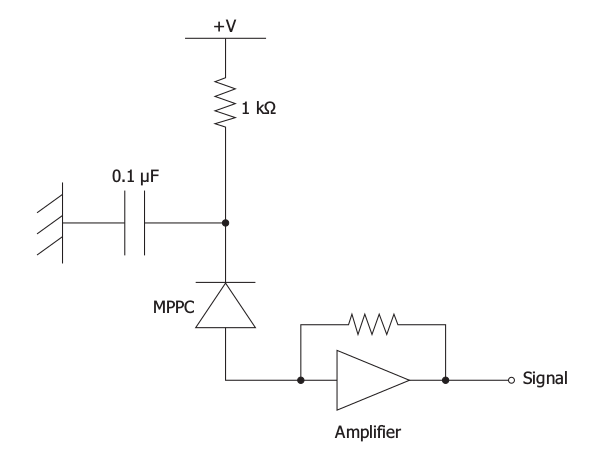
\includegraphics[width=\textwidth]{3DesignPrinciples/32Tritium_detector/ElectronicSchemePCBSiPM.png}  
    \caption{\label{subfig:ElectronicSchemePCBSiPM}}
    \end{subfigure}
    \hfill
 \caption{a) Electronic board used to provide the SiPM bias voltage and to read the SiPM output signal. b) Electronical scheme in which this PCB is based.}
 \label{fig:PCBSiPM}
\end{figure}
This PCB, shown in Figure \ref{fig:PCBSiPM}, was feed at $\pm6~\volt$ using the voltage source ISOTECH, model IPS-4303 \cite{VoltageSourceISOTECH} and the SiPM was feed using the electrometer KETHLEY, model 6517B \cite{VoltageSourceKethley}, that achieves a resolution of $1~\milli\volt$, low enough to ensure that voltage variations do not affect the SiPM gain. The output signal was connected to an oscilloscope, model WwaveRunner 625Zi from TELEDYNE LECROY \cite{OscilloscopeIFIMED} that recorded the data which were subsequently analized by ROOT\footnote{ROOT is a framework for data processing, based on C ++ and object-oriented technology, developed at CERN and widely used in nuclear and particle physics.} scripts.